%Start with a Clear Heading: Begin your report with a heading that clearly states "Background" or "Introduction" to let readers know where to find this information.

%Provide an Overview: Begin by providing a brief overview of the project, including its title and purpose. You can mention what the project aims to achieve or the problem it intends to address.

%Contextualize the Project:

%Explain the broader context in which the project exists. Discuss any relevant industry trends, challenges, or issues that the project is responding to.
%Mention any external factors or events that have prompted the need for the project.
%If the project is part of a larger initiative or program, briefly introduce that program and explain how your project fits into it.
%Historical Background:

%Provide historical information if relevant. Explain how this project came into consideration, including any past efforts or developments leading up to it.
%If there are key milestones or events that are crucial to understanding the project's origins, mention them.
%State the Problem or Opportunity:

%Clearly state the problem or opportunity your project aims to address. Use data or facts to support your claims.
%If applicable, describe the significance of the problem or opportunity, such as its impact on the organization, stakeholders, or the community.
%Objective and Scope:

%Outline the specific objectives and scope of the project. What are you trying to achieve, and what are the boundaries or limitations of the project?
%Explain why these objectives are important and how they relate to solving the identified problem.
%Review of Relevant Literature:

%If there's existing research or literature relevant to your project, briefly mention it. This shows that you've conducted a literature review and are building upon prior knowledge.
%Highlight any gaps or areas where your project adds value or addresses shortcomings in existing research or practices.
%Cite Sources: Make sure to provide proper citations for any data, statistics, or information you use in this section.

%Keep it Concise and Engaging: While providing all necessary information, avoid making the background section overly long. Keep it engaging and focused on the most crucial information.

%Transition to the Next Sections: Conclude the background section by smoothly transitioning into the next sections of your report, such as the objectives, methodology, or project plan.

%Remember to tailor the background section to your specific project and audience. Your goal is to provide a comprehensive but concise overview that sets the stage for the reader to understand the significance and context of your project.

\chapter{Background}
\label{chap3}

\section{What are glitch attacks?}

Glitch attacks can be divided into two main categories: invasive (e.g., decapsulating the chip\cite{intro_to_hw_hacking}) and non-invasive attacks (e.g., electromagnetic fault injection (EMFI), voltage- and clock-glitching). Often times software and firmware security measures can only protect against non-invasive glitches, as protecting from invasive glitches often require hardware modifications\cite{glitchresistor}. Due to the nature of invasive attacks, it is beyond the scope of this project to defend against them. These often aim at tampering with Read-Only Memory (ROM) or Boot-loaders on Printed Circuit Boards (PCBs), and are not effective against more complex systems like a Central Processing Unit (CPU) or a System on Chip (SoC). 

Non-invasive glitches can be performed as long as an attacker has access to a device. However, there is quite a lot of procedural vulnerability discovery that has to be done before an attack can be performed. In the case of EMFI the chip has to be repeatedly exposed to electromagnetic interference during execution, to then determine which areas are most vulnerable to attacks\cite{emfi_injection}. An example of this being performed on the BCM2837 SoC can be seen in \autoref{fig:emfi_map}\cite{emfi_injection}. 

Voltage- or clock-glitching can be performed as long as there is some way to access these signals externally. Voltage-glitching often requires the removal of power filtering capacitors to gain more fine-grained control over a processor's voltage input. However, both of these methods require very precise timing by an attacker. This is why specialized tools such as the \textit{ChipWhisperer}\cite{chipWhisperer} are needed, as they allow extremely accurate fault-injection. These days it is also possible to perform effective glitch attacks with simple components in conjunction with a cheap Field Programmable Gate Array (FPGA) which outputs precise triggers\cite{hole_in_soc}. 

\begin{figure}[h!]
    \centering
    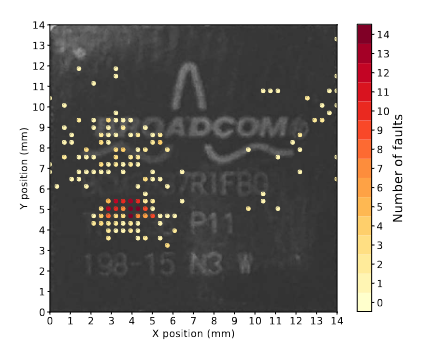
\includegraphics[scale=0.5]{docs/images/emfi_error_map.png}
    \caption{EMFI BCM2837 sensitivity map (dot size is not corralated with probe size.)\cite{emfi_injection}.}
    \label{fig:emfi_map}
\end{figure}

Voltage-glitching is performed by momentarily dropping the supply voltage during execution of critical operations. Clock-glitching is performed by altering clock timing to violate setup and hold time requirements of the hardware\cite{intro_to_FI}. The results of glitching cannot always be predicted, however they mainly result in skipped or repeated CPU instructions, incorrect evaluation of CPU instructions or corrupt reads from memory devices\cite{intro_to_FI}. In general these faults can occur at any stage in the execution pipeline. A typical application for these types of glitches is to skip some sort of signature verification in a bootloader or other security module. The code snippet in \autoref{fig:glitch_code} shows how it could be used to bypass secure-boot.

\begin{figure}
\begin{lstlisting}[language=C]
...
if (signature_match) // <- Glitch here
{
    load_runtime_firmware();
}
else 
{
    do_not_load_runtime_firmware();
}
...
\end{lstlisting}
\caption{Glitching past signature validation in secure-boot.}
\label{fig:glitch_code}
\end{figure}

% Glitch attacks have over recent years become a more common and greater threat. Due to the nature of how these attacks are carried out, they are often a very affordable way to exploit hardware. Attackers have easy access to open source resources like the the 'ChipWhisperer Lite' which allows for easy access to hardware glitching tools as well as side channel analysis\cite{chipWhisperer}. In addition to this, FPGAs can be used to inject precisely timed faults as long as an attacker has access to the supply voltage or clock on a chip\cite{hole_in_soc}. 

\section{The need for glitch protection}

Within the world of CPU design the two biggest architectures are ARM and x86 (produced by Intel and AMD). Most of the devices we us every day has one of these types of chips inside them, and because of this they also implement several security features to prevent glitch attacks. For ARM processors this includes among other things the \textit{TrustZone} which provides hardware-enforced isolateion between trusted and non-trusted software, as well as built in physical attack protection\cite{arm}. The 12th gen x86 processors produced by Intel have a Tunable Replica Circuit (TRC), which uses hardware-based sensors to explicitly detect circuit-based timing failures that occur as the result of an attack\cite{intel}.  

Unfortunately, for many years the world of CPU design has been hidden from the public due to the strict secrecy producers have around their products. While this limits what the general public can know, it also means that a potential hacker would have a much harder time if they wished to exploit how the ISA of a chip is designed. Due to the nature of open source projects, this is a larger vulnerability for products based on a RISC-V architecture. An example of direct exploitation of the architecture was shown during the 'DEFCON' conference in 2019\cite{isa_exploit}. Here it was demonstrated that triggering an exception during boot of a RISC-V chip would lead to an 'exception loop'. This was because the Machine Trap Vector (MTVEC) had no base address before boot (e.g., it was set to 0x0). Pointing to this address is permitted in the ISA, and doing so will trigger an exception. This means that triggering an exception before boot leads to the exception handler pointing to an illegal address, which again triggers an exception and this continues forever. Handling of exceptions happens first at the highest privilege mode (Machine mode), which means that the chip is also stuck in this mode. 

The RISC-V architecture is designed with some key security features in mind. One of these are the previously mentioned privilege levels. These are in descending order: machine (M-mode), hypervisor (H-mode), supervisor (S-mode) and user mode (U-mode). A higher privilege mode can access all the functions used in a lower privilege mode\cite{source2}. Other key security features in the RISC-V architecture are the physical memory protection (PMP), which controls memory accesses, and the use of a trusted execution environment (TEE). The TEE is meant to ensure that code and data loaded into this environment are protected with respect to confidentiality and integrity. However, as shown in (Nashimoto et al. 2020) the integrity of TEEs can also be bypassed using clock-glitching\cite{source2}.

%\section{Previous Approaches to glitch protection}
\section{CV32E40S by the OpenHW group}
\label{sec:cv32}

The previously mentioned security measures do a decent job at protecting hardware against malicious attacks. However, the need for more security features has been required and therefore the \textit{OpenHW} group developed the \textit{CV32E40S}. This is a 4-stage in-order 32-bit RISC-V processor core with the main intention of ensuring secure operation\cite{cv32e40s_manual}. This core has the same privilege modes and PMP as described to ensure a TEE. There are however implemented extra security features and an Instruction Set Extension (ISE), \textit{Xsecure}. The CV32E40S started out as a fork of the CV32E40P which is another RISC-V processor made by the OpenHW group. The top-level block diagram of the cores is shown in \autoref{fig:core_comparison_block}. From the figure we can see that the main difference on the top level is the PMP and the Physical Memory Attribution (PMA), which allows for compile time attribution of the physical memory map.

\begin{figure}[h!]
\centering
    \subfigure[CV32E40P\cite{cv32e40p_manual}.]{%
    \label{fig:cv32e40p_block}%
    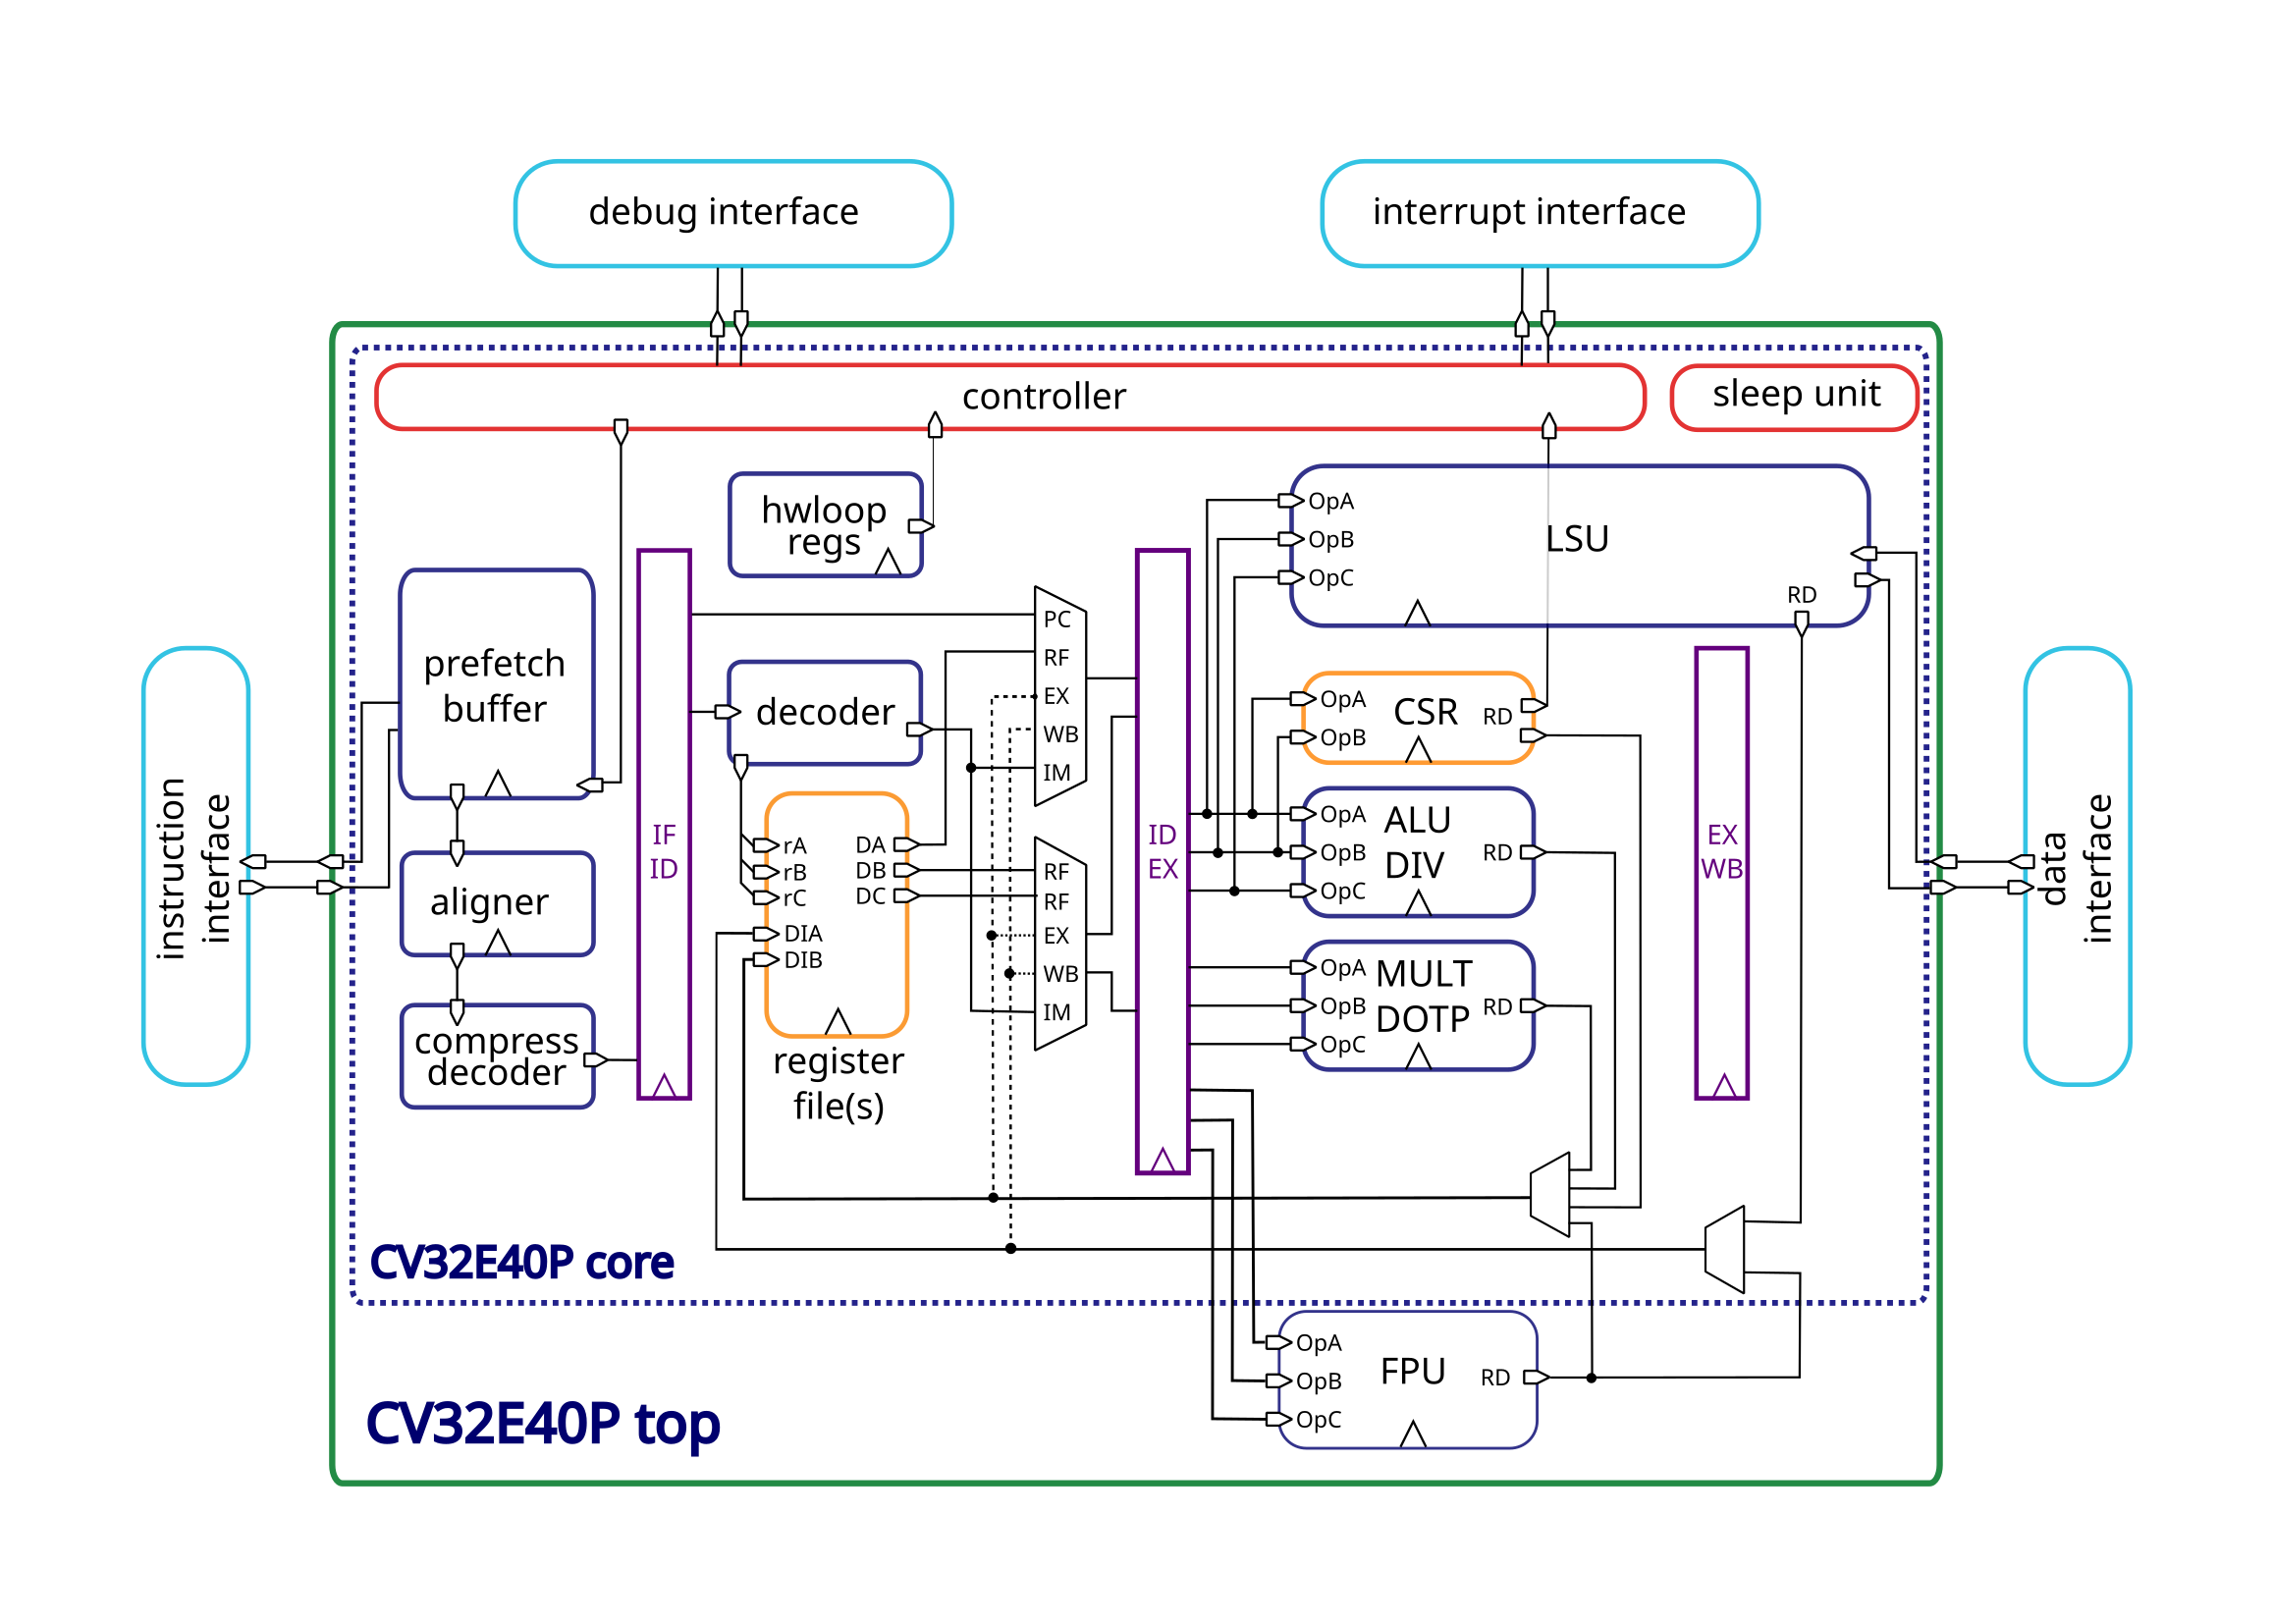
\includegraphics[width=0.47\textwidth]{docs/images/CV32E40P_Block_Diagram.png}}%
    \qquad
    \subfigure[CV32E40S\cite{cv32e40s_manual}.]{%
    \label{fig:cv32e40s_block}%
    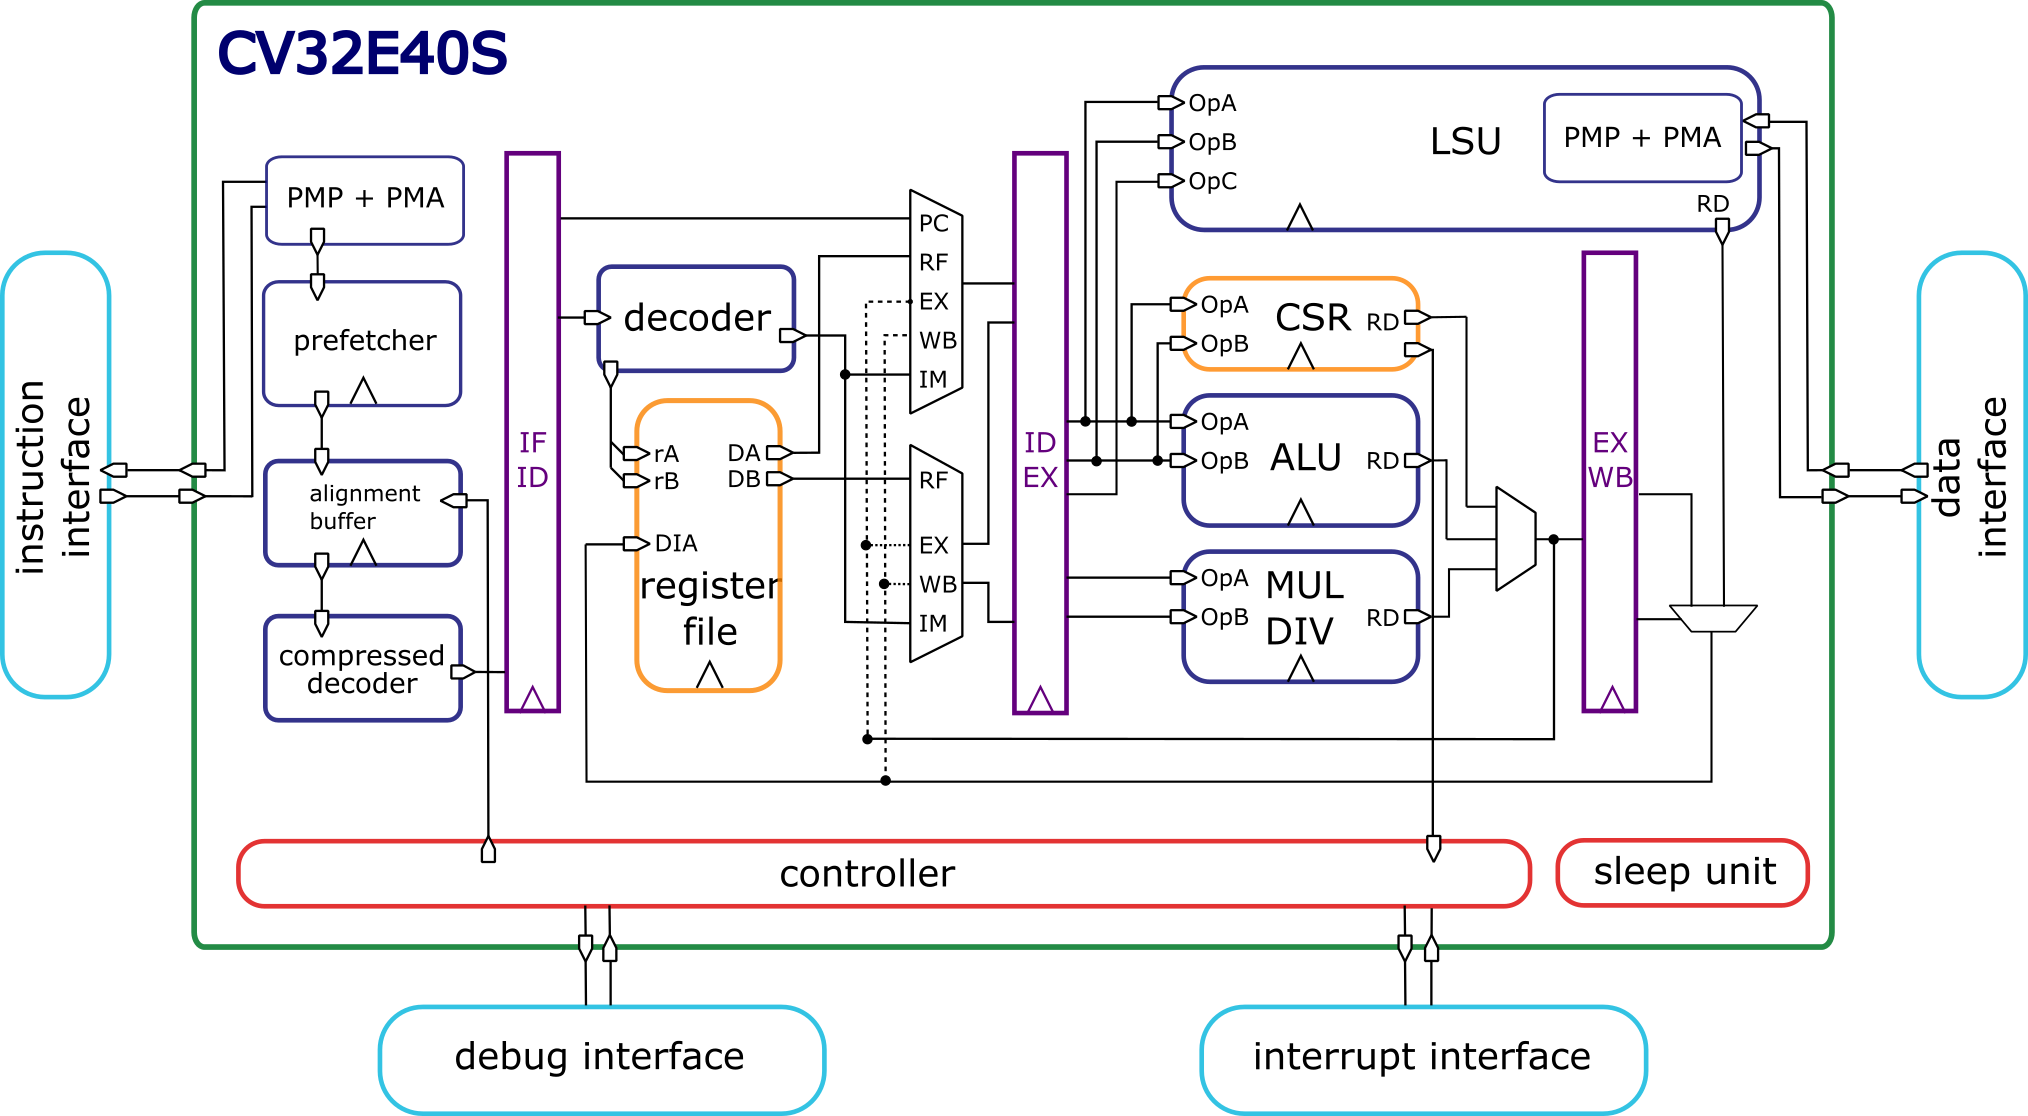
\includegraphics[width=0.47\textwidth]{docs/images/CV32E40S_Block_Diagram.png}}%
    \caption{Comparison of Top-Level Block Diagram for CV32E40S and CV32E40P.}
    \label{fig:core_comparison_block}
\end{figure}

\subsection{Xsecure Extension}

\textit{Xsecure} is an ISE that adds extra security functionality within many of the different sub modules of the core. These security features are meant to deter side-channel attacks through the use of \textit{data independent timing}, \textit{dummy instruction insertion} and \textit{random instructions}\cite{cv32e40s_manual}. While these features will increase execution time, they cannot easily be removed with the use of a dual core setup. This is because preventing side-channel attacks is less about redundancy and more about making the power usage or execution time of a processor unpredictable. 

The extension also adds specific security features to prevent glitch attacks. These include: \textit{Register file ECC}, \textit{Hardened PC} and \textit{Hardened CSRs} among other things. These features can potentially be removed in favour of a dual core lock-step mechanism. Removing only these features without also affecting the core as a whole is quite complicated. However, to give some insight into the resource usage and added execution time for these sub-modules, the core has been simulated and synthesized both with and without \textit{PC Hardening}. When simulation of the core is done, a simple \textit{hello-world} example is run, shown in \autoref{app:helloworldC}. From simulation of both cores it is shown that the core requires \textbf{9} extra clock cycles when using \textit{PC-hardening} as can be seen in \autoref{tab:simulation_cc}. The generated assembly code for this program consists of \textit{11875} instructions. From the documentation about the core, it is explained that \textit{jumps} as well as \textit{branches} that are not taken will require one extra clock cycle due to \textit{PC-hardening}. 

\begin{table}[h]
\centering
\caption{Number of clock cycles needed to simulate the program in \autoref{app:helloworldC} with and without \textit{PC-Hardening}.}
\label{tab:simulation_cc}
\begin{tabular}{cc}
\toprule 
With PC-Hardening & Without PC-Hardening \\
\midrule
\rowcolor{black!20} 18289 & 18280 \\
\bottomrule
\end{tabular}
\end{table}

\begin{figure}
    \centering
    \includegraphics{}
    \caption{Caption}
    \label{fig:enter-label}
\end{figure}

From synthesis of both cores it can also be seen that the \textit{PC-Hardening} will add a bit to the total resource usage. The results of synthesis can be seen in \autoref{tab:synth_ppa}.

\begin{table}[h]
\centering
\caption{Synthesized resource usage with and without \textit{PC-Hardening}.}
\label{tab:synth_ppa}
\begin{tabular}{ccc}
\toprule 
& With PC-Hardening & Without PC-Hardening \\
\midrule
\rowcolor{black!20} \textbf{area[$pm^2$]} & 63164.38 & 61757.916 \\
\textbf{power[$W$]} & 1.12163mW & 1.10450mW \\
\rowcolor{black!20} \textbf{LUTs} & -- & -- \\
\bottomrule
\end{tabular}
\end{table}



%One of the implemented features is the \textit{Hardened Program Counter} (Hardened PC). The main idea behind this feature is to check that during sequential operation, the PC in the Instruction Fetch (IF) stage has the correct value as the one determined by the compressed/uncompressed state of the instruction in the Instruction Decode stage. In addition to this it checks that the target for a branch or jump instruction is correct during non-sequential operation. 

% \textbf{PC hardening step by step}
% \begin{itemize}
%     \item Set expected address for sequential updates based on address in ID and type of instruction (compressed + 2 / uncompressed + 4)
%     \begin{itemize}
%         \item \textbf{Uncompressed instructions}: Standard RISC-V instructions are 32 bits long. These ar eoften refferd to as uncompressed and adhere to the base integer instruction format. 
%         \item \textbf{Compressed instructions}: Compressed instructions are 16 bits. These often represent frequently used instructions at half the space. 
%     \end{itemize}
%     \item The control flow address is chosen based on flopped value comping from the PC-MUX. If the PC-MUX is glitched, this mux may choose the wrong address and an address comparison error is likely to happen. 
%     \item Choose which address to check vs the IF PC: Sequential or Control flow.
%     \item Instructions are 16-bit aligned since the core supports compressed instructions. 
%     \item Address comparison is only valid the cycle after the PC is set or the cycle after an instruction goes from IF to ID. 
% \end{itemize}

\section{Limitations of glitch protection and proposed solution}
\label{sec:limits}

Because glitch protection has gained more attention over recent years, several methods are implemented by different CPU producers. However, many of these security features all have some common limitations. For instance the coverage of protection can often be incomplete. This means that designers often only focus on the most critical glitches, and can therefore sometimes overlook seemingly insignificant glitches that might break the system. For instance, a designer could implement a robust check to see whether the program counter has been modified during execution. However if an attacker glitches the program counter on boot, it could go undetected by the checker mechanism. 

In general glitch protection mechanisms will add to both the area and power consumption of a chip. Often the added area also comes from components that are logically redundant. In addition there will be a lot of latency added to the system. 


\begin{itemize}
    \item High logic cost 
    \item Slower execution of certain pipeline stages
    \item Lower throughput 
    \item A typical way of doing fault injection is though EMFI attacks which target larger components like caches or other memory components.
    How can we prevent these? Comparing the state of the entire chache is not viable, and thus we must allow a fault to persist in 
    memory untill it is read or used in one of the cores.
\end{itemize}

\textbf{I NEED TO SIMULATE THE CORE WITH AND WITHOUT PC-HARDENING AND CSR-HARDENING TO SEE THE DIFFERENCE IN PPA}
\textbf{I need to create a c program that has some code that is easily glitchable that represents a real world safety feature. This could be an infinite while loop, where the aim is to break out of this loop using a glitch. To achieve this I can either make a module whose sole purpose is to glitch a register and then make this glitchin happen radomly. Or i can induce som form of clock-glitching. This might not be possible in simulation as the setup / hold times will not be realistic. Voltag eglitching is also not possible as I dont havee access to the supply voltage of the system.}

\textbf{TODO:}
\begin{itemize}
    \item Run simulation of core with and without xsecure extension 
    \begin{itemize}
        \item Find out where the Xsecure extension is being enabled from. Maybe this is in the documentation. 
    \end{itemize}
    \item Run synthesis of core (with and without xsecure extension) 
    \begin{itemize}
        \item Power estimation 
        \item LUTs and Area 
    \end{itemize}
    Detail the program that is running when these tests are performed(mostly for simulation)
    \item Detail how dual cores could work in theory to improve things 
    \item Describe the tests that will be performed to simulate glitching
    \item Describe test program that will be running on the core (an infinite while loop to simulate some form of security check)
    \item Describe the odule that will be implemented to simulate a glitch attack.
\end{itemize}

\section{Simulation data}
\subsection{Clock cycles}
With PC hardening disabled: 6 cycles

\subsubsection{Hardened CSR}

\section{The dual core proposition}
\section{Rationale for this study}

